\documentclass[../../../topic_calculus]{subfiles}

\begin{document}

\sectionline
\section{二変数関数のグラフ}
%\marginnote{\refbookA p163〜166}

2変数関数$f(x, y)$が与えられたとき、変数$x,\,y$を自由に動かして点$(x, y, f(x,y))$を$xyz$空間でプロットして得られる曲面を$z= f(x, y)$の\keyword{グラフ}という。

\br

$f(x,y)$が地点$(x, y)$の標高の場合は、この$z=f(x,y)$のグラフが表す曲面はこの野山の地表にほかならない。
\begin{itemize}
  \item 2変数関数$f(x, y)$をグラフで可視化すると、野山の形状になる
  \item 野山の形状から標高を考えると、2変数関数$f(x, y)$になる
\end{itemize}

\subsection{$z = x^2 + y^2$のグラフ}

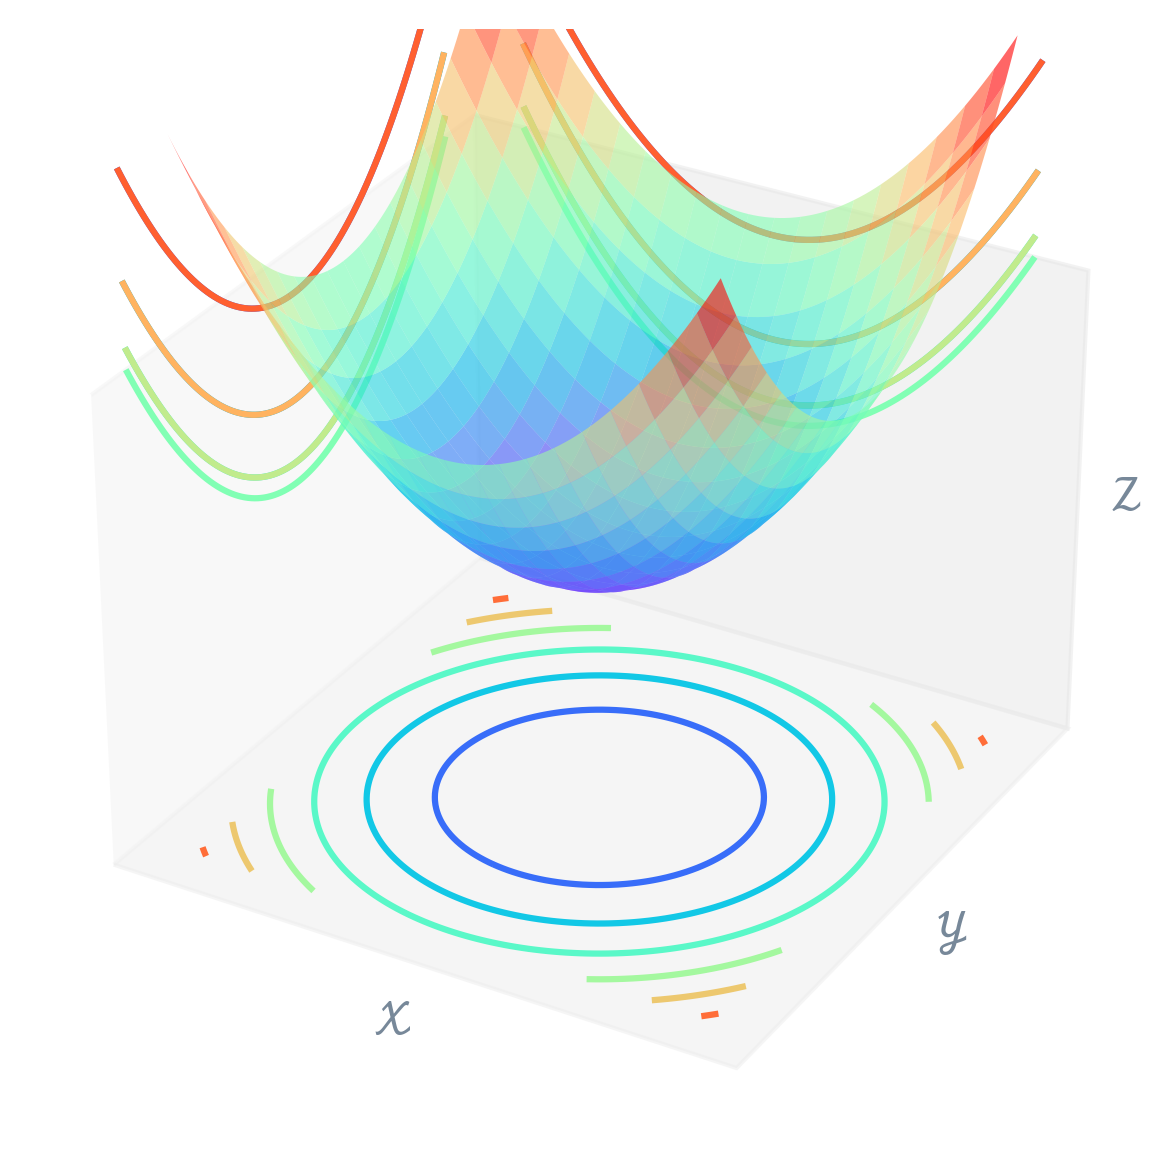
\includegraphics{../python/graph_x-pow2-add-y-pow2_01.png}

\begin{itemize}
  \item {\bfseries $xy$平面($z=0$)} 円$x^2 + y^2 =0$
  \item {\bfseries $xz$平面($y=0$)} 下に凸の放物線$z=x^2$
  \item {\bfseries $yz$平面($x=0$)} 下に凸の放物線$z=y^2$
\end{itemize}

「曲面を見る」堅実な方法は、\keyword{断面図(切り口)}を順に見ることである。

\begin{enumerate}
  \item $y=0$とすると、断面が$xz$平面内の放物線$z=x^2$になる
  \item $y=1$とすると、$z=x^2+1$となり、これは$z=x^2$のグラフを$1$だけ高くした放物線
  \item $y=2$とすると、$z=x^2+4$となり、放物線がさらに高くなる
\end{enumerate}

こうして、$y=\text{\bfseries 定数}$とした断面図をつなぎ合わせることで曲面の姿をつかむことができる。

\subsection{$z = x^2 - y^2$のグラフ}

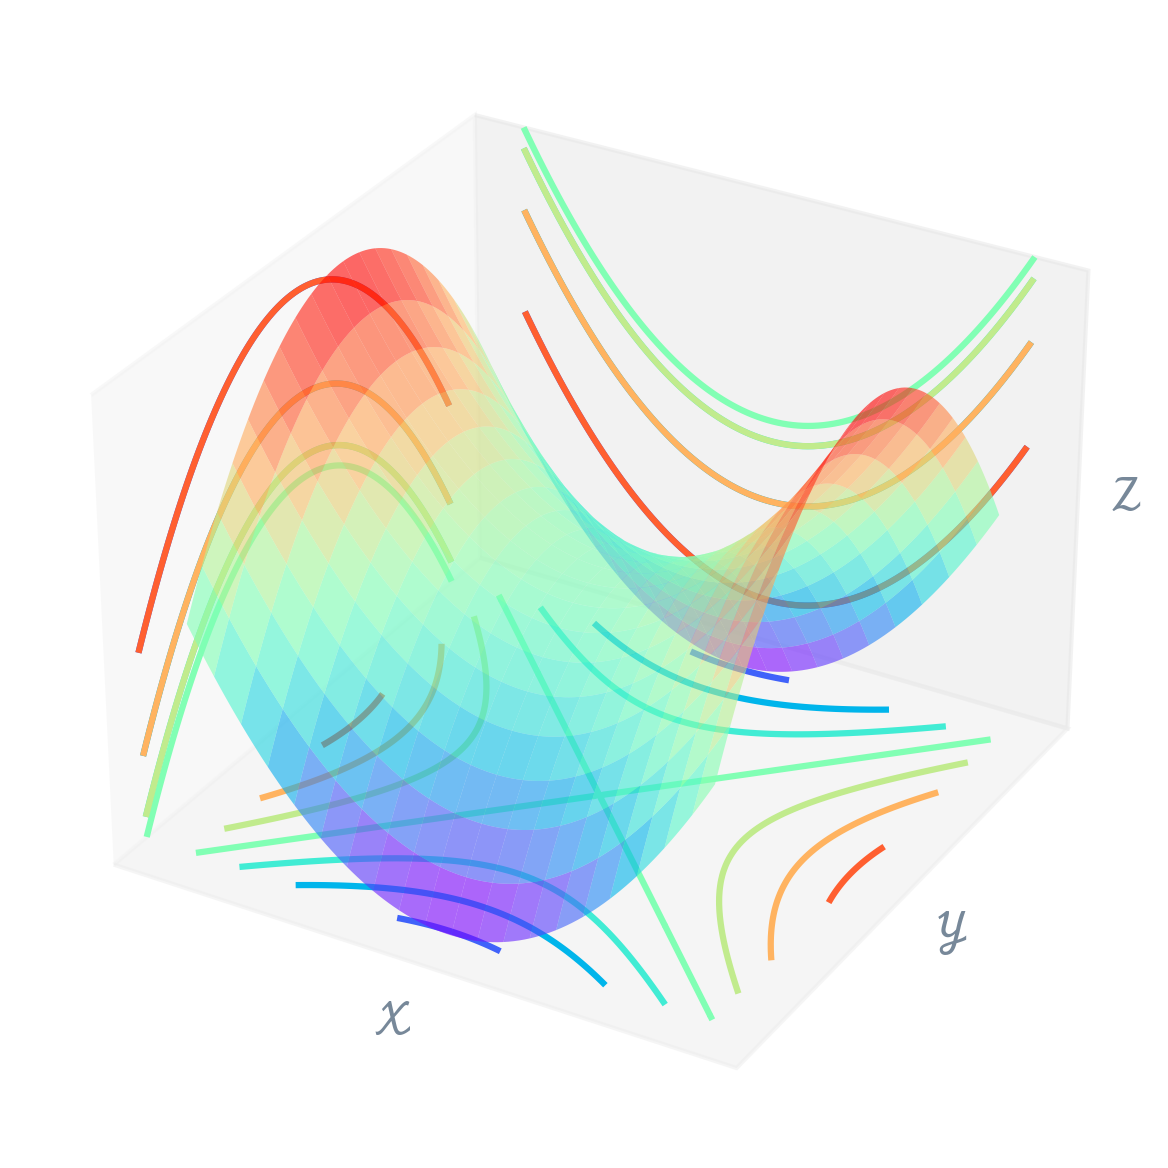
\includegraphics{../python/graph_x-pow2-sub-y-pow2_01.png}

\begin{itemize}
  \item {\bfseries $xy$平面($z=0$)} 双曲線$x^2 - y^2 =0$
  \item {\bfseries $xz$平面($y=0$)} 下に凸の放物線$z=x^2$
  \item {\bfseries $yz$平面($x=0$)} 上に凸の放物線$z=-y^2$
\end{itemize}

下に凸の放物線(吊り下げたひも)の各点に、上に凸の放物線(針金)を順に貼り付けていくと、$z=x^2-y^2$のグラフが得られる。

\end{document}
